%======================================================================
% OPTION A — pgfplots scatter figures: routing time & TNS impact
%======================================================================

\begin{figure}[t]
    \centering
    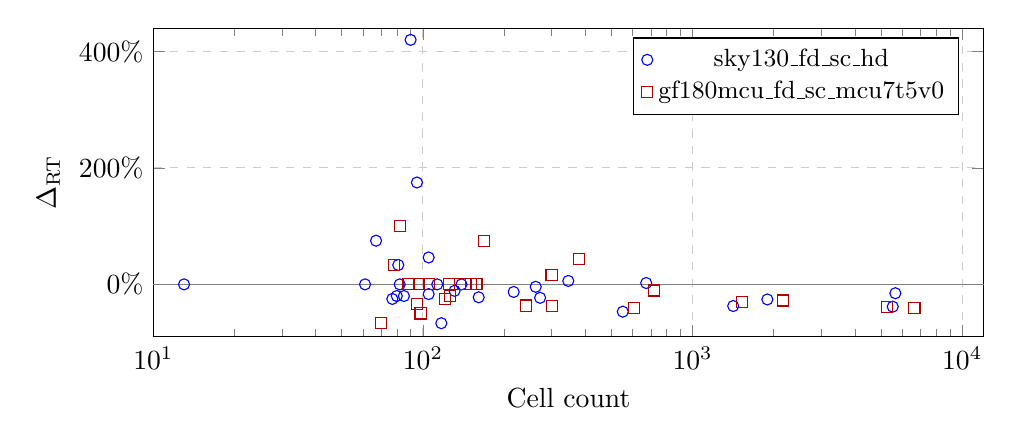
\begin{tikzpicture}
        \begin{semilogxaxis}[
            width=\columnwidth, height=5.5cm,
            xlabel={Cell count},
            ylabel={$\Delta_{\mathrm{RT}}$},
            ylabel style={align=center},
            xmin=10, xmax=12000,
            ymin=-90, ymax=440,
            yticklabel={\pgfmathprintnumber{\tick}\%},
            grid=major, grid style={dashed,gray!40},
            legend pos=north east,
            legend style={font=\small},
            mark size=2pt,
            clip=false,
            ]
            % zero line
            \draw[gray,thin] (axis cs:10,0) -- (axis cs:12000,0);

            \addplot[only marks, mark=o, blue] coordinates {
            (13,0.0)  % s27
            (61,0.0)  % s298
            (67,75.0)  % s386
            (77,-25.0)  % s420
            (80,-20.0)  % s349
            (81,33.3)  % s382
            (82,0.0)  % s344
            (85,-20.0)  % s444
            (90,420.0)  % s400
            (95,175.0)  % s526
            (105,46.2)  % s641
            (105,-16.7)  % s713
            (113,0.0)  % s1196
            (117,-66.7)  % s510
            (131,-11.1)  % s820
            (139,0.0)  % s832
            (161,-22.2)  % s838
            (217,-13.0)  % s953
            (262,-4.2)  % s1196b
            (272,-23.1)  % s1238
            (346,5.9)  % s1423
            (551,-46.9)  % s9234
            (673,2.3)  % s5378
            (1415,-37.2)  % s13207
            (1894,-25.9)  % s15850
            (5526,-38.3)  % s38584
            (5651,-15.2)  % s35932
            };
            \addlegendentry{sky130\_fd\_sc\_hd}
            \addplot[only marks, mark=square, red!70!black] coordinates {
            (70,-66.7)  % s298
            (78,33.3)  % s386
            (82,100.0)  % s420
            (88,0.0)  % s349
            (89,0.0)  % s344
            (95,-33.3)  % s382
            (97,0.0)  % s400
            (98,-50.0)  % s444
            (105,0.0)  % s526
            (121,-25.0)  % s1196
            (125,0.0)  % s641
            (126,-20.0)  % s713
            (137,0.0)  % s510
            (151,0.0)  % s820
            (158,0.0)  % s832
            (169,75.0)  % s838
            (241,-36.4)  % s953
            (300,15.4)  % s1196b
            (301,-36.8)  % s1238
            (378,42.9)  % s1423
            (606,-40.9)  % s9234
            (719,-10.5)  % s5378
            (1529,-30.5)  % s13207
            (2158,-27.7)  % s15850
            (5255,-38.9)  % s35932
            (6650,-40.1)  % s38584
            };
            \addlegendentry{gf180mcu\_fd\_sc\_mcu7t5v0}
        \end{semilogxaxis}
    \end{tikzpicture}
    \caption{Per-design detailed-routing runtime change of \textsc{ScanOpt}
    (\emph{opt}) vs.\ placement-aware baseline (\emph{basic}) as a function of
    cell count. No consistent trend with design size; \emph{s27} on gf180mcu
    omitted (basic runtime rounds to 0s, undefined \% change).}
    \label{fig:scanopt_scatter_rt}
\end{figure}

\begin{figure}[t]
    \centering
    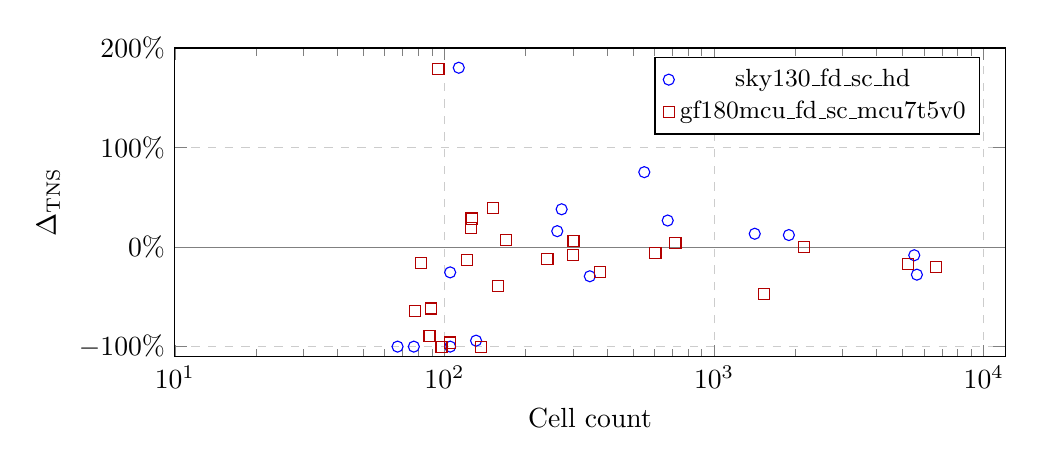
\begin{tikzpicture}
        \begin{semilogxaxis}[
            width=\columnwidth, height=5.5cm,
            xlabel={Cell count},
            ylabel={$\Delta_{\mathrm{TNS}}$},
            ylabel style={align=center},
            xmin=10, xmax=12000,
            ymin=-110, ymax=200,
            yticklabel={\pgfmathprintnumber{\tick}\%},
            grid=major, grid style={dashed,gray!40},
            legend pos=north east,
            legend style={font=\small},
            mark size=2pt,
            clip=false,
            ]
            % zero line
            \draw[gray,thin] (axis cs:10,0) -- (axis cs:12000,0);

            \addplot[only marks, mark=o, blue] coordinates {
            (67,-100.0)  % s386
            (77,-100.0)  % s420
            (105,-100.0)  % s641
            (105,-25.4)  % s713
            (113,180.2)  % s1196
            (131,-94.0)  % s820
            (262,16.0)  % s1196b
            (272,38.0)  % s1238
            (346,-29.3)  % s1423
            (551,75.3)  % s9234
            (673,26.7)  % s5378
            (1415,13.4)  % s13207
            (1894,12.1)  % s15850
            (5526,-8.2)  % s38584
            (5651,-27.7)  % s35932
            };
            \addlegendentry{sky130\_fd\_sc\_hd}
            \addplot[only marks, mark=square, red!70!black] coordinates {
            (78,-63.9)  % s386
            (82,-15.9)  % s420
            (88,-89.5)  % s349
            (89,-61.7)  % s344
            (95,178.9)  % s382
            (97,-100.0)  % s400
            (98,-100.0)  % s444
            (105,-95.9)  % s526
            (121,-12.8)  % s1196
            (125,19.1)  % s641
            (126,28.7)  % s713
            (137,-100.0)  % s510
            (151,39.3)  % s820
            (158,-39.0)  % s832
            (169,7.4)  % s838
            (241,-12.0)  % s953
            (300,-7.7)  % s1196b
            (301,6.3)  % s1238
            (378,-25.2)  % s1423
            (606,-5.7)  % s9234
            (719,4.2)  % s5378
            (1529,-47.5)  % s13207
            (2158,-0.3)  % s15850
            (5255,-17.2)  % s35932
            (6650,-20.1)  % s38584
            };
            \addlegendentry{gf180mcu\_fd\_sc\_mcu7t5v0}
        \end{semilogxaxis}
    \end{tikzpicture}
    \caption{Per-design total negative slack (TNS) change of \textsc{ScanOpt}
    (\emph{opt}) vs.\ placement-aware baseline (\emph{basic}) as a function of
    cell count. No consistent trend with design size; designs with zero
    baseline TNS (no setup violations under \emph{basic}) are omitted,
    undefined \% change.}
    \label{fig:scanopt_scatter_tns}
\end{figure}
